\chapter{前言}
\renewcommand{\baselinestretch}{10.0} %設定行距
\pagenumbering{arabic} %設定頁號阿拉伯數字
\setcounter{page}{1}  %設定頁數
\fontsize{14pt}{2.5pt}\sectionef
\section{研究動機}
機器學習與各領域結合的應用越來越廣泛,在機電系統採用強化學
習是為了讓機電系統的控制達到最佳化。本專題希望利用現代機器學習和模擬技術來建立一個虛擬的足球機系統作為訓練模型,將實體機器轉移到虛擬環境進行模擬,為了找到適合的訓練參數,因此將模型簡化後再進行測試各種參數的調整,透過不斷的訓練來得到一個優化過的對打系統,以下是成品圖。
\\

\begin{figure}[hbt!]
\begin{center}
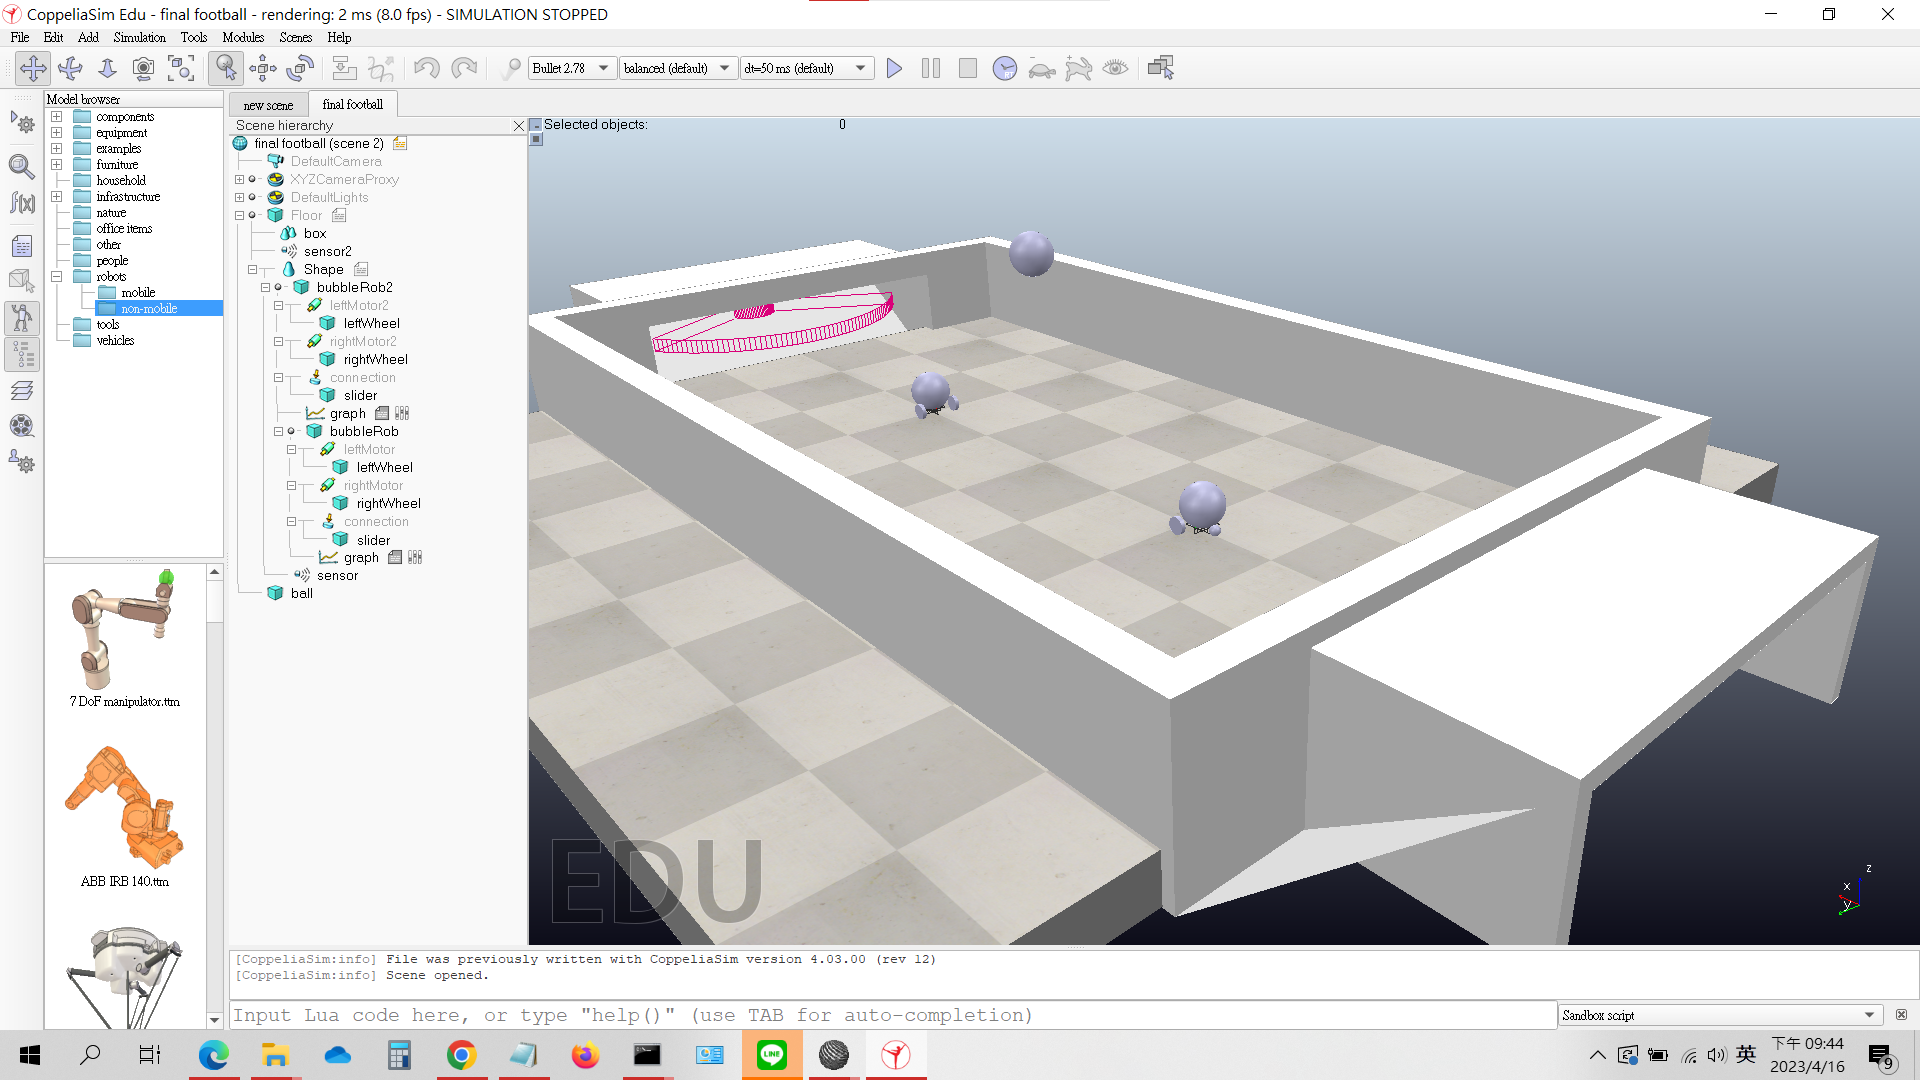
\includegraphics[angle=0,width=17cm]{足球機}
\caption{\Large 模擬情形}\label{fig.足球機}
\end{center}
\end{figure}
\newpage



\section{製作過程}

1.先繪製球檯\\
\begin{figure}[hbt!]
\begin{center}
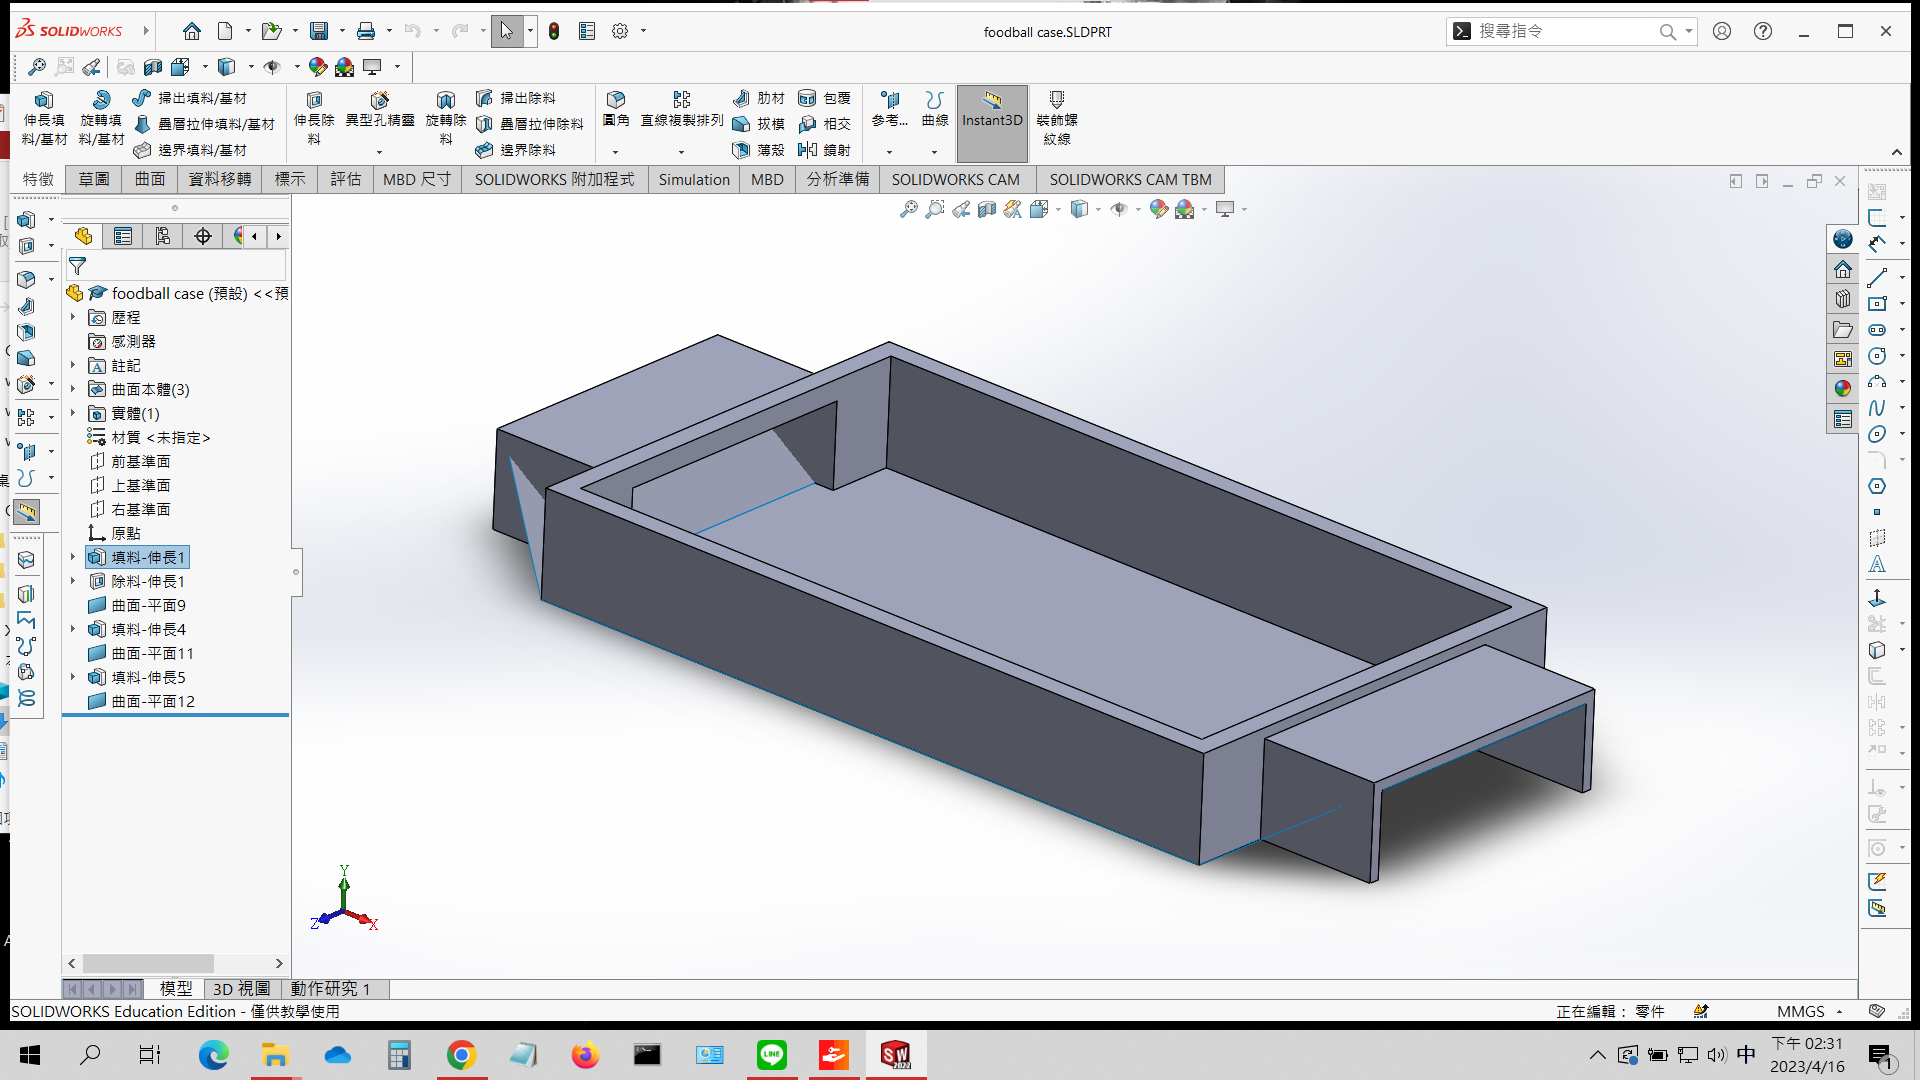
\includegraphics[angle=0,width=15cm]{football stage}
\caption{\Large 球檯}\label{fig.football stage}
\end{center}
\end{figure}

2. 接著增加以 lua 腳本控制使 bubbleRob 可以前後左右移動 sim.getObjectHandle 這個函
式在 coppeliasim4.3.0 版本被淘汰了但還是可以使用,後來則改為 sim.getObject
去做使用在後面感測器腳本已做改善,並使復健名稱相互對應則可執行。\\

\begin{figure}[hbt!]
\begin{center}
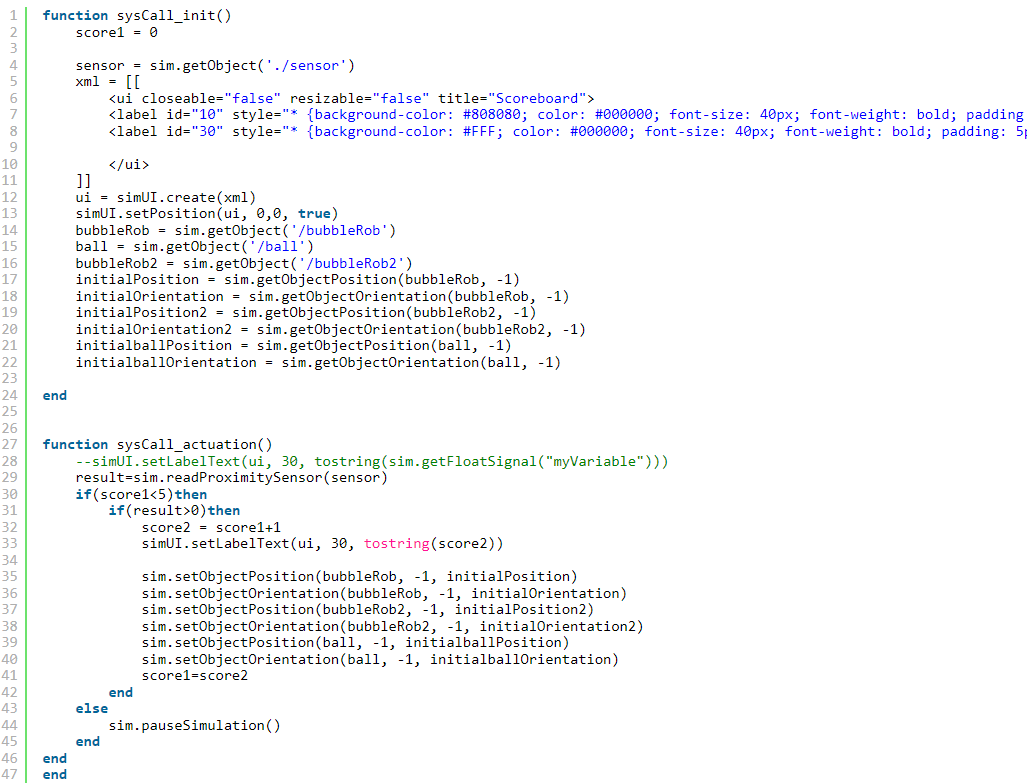
\includegraphics[angle=0,width=15cm]{感測器腳本}
\caption{\Large 感測器Lua}\label{fig.感測器腳本}
\end{center}
\end{figure}
\newpage

3.加入記分板並進行連線\\
\begin{figure}[hbt!]
\begin{center}
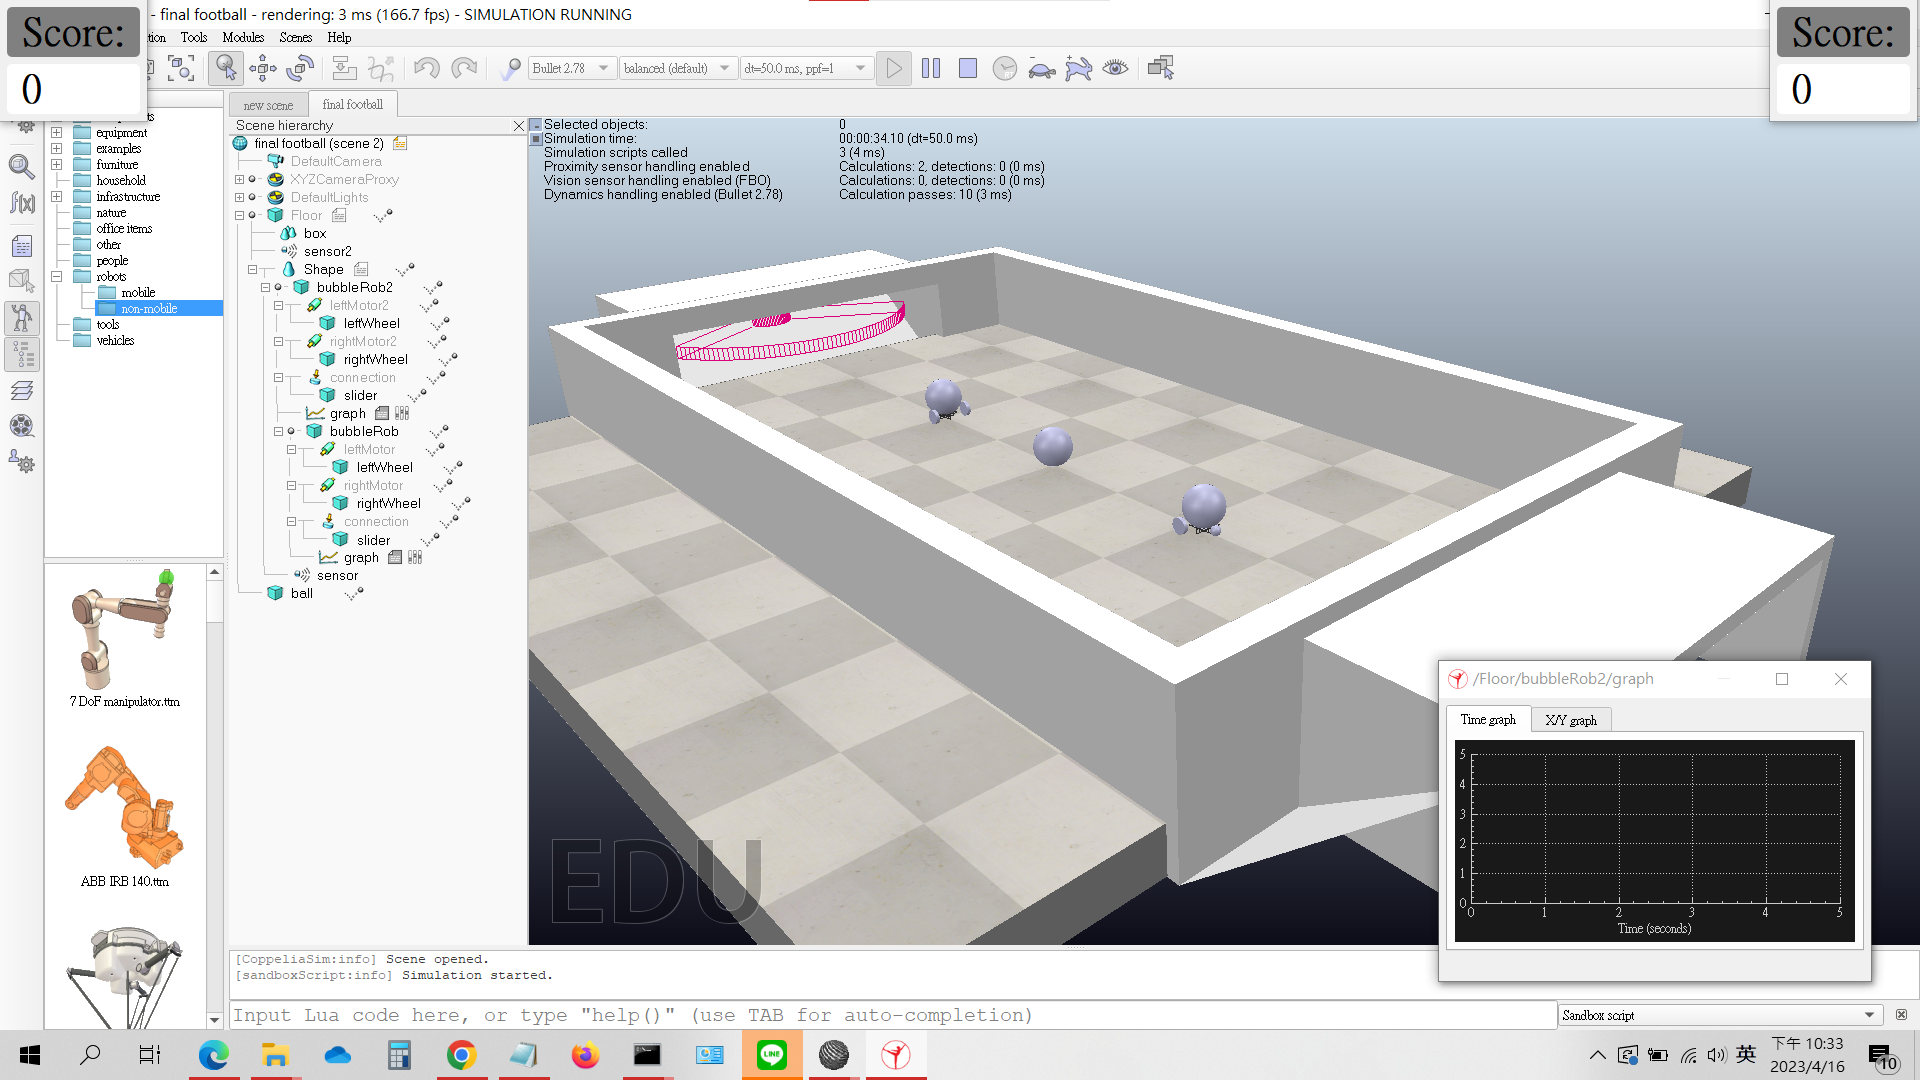
\includegraphics[angle=0,width=15cm]{連線模擬}
\caption{\Large 模擬情形}\label{fig.連線模擬}
\end{center}
\end{figure}
\newpage
 
 \chapter{環境設定}
\renewcommand{\baselinestretch}{10.0} %設定行距
\pagenumbering{arabic} %設定頁號阿拉伯數字
\setcounter{page}{1}  %設定頁數
\fontsize{14pt}{2.5pt}\sectionef

\section{未來展望}
此專題希望能利用現有完成的機械學習的算法,能發展成虛擬訓練,再將訓練完的機器學習應用到虛擬環境或是實體機電系統,並透過伺服器將影像串流提供玩家網頁介面進行遠端操控,同時提供多人觀看及時的比賽影像,將整個冰球機的控制和使用者間有更完善串聯,機電系統的部分達到最優化控制和虛實整合的應用。
\section{規則說明}
 Pong game 的遊戲規則簡單,透過擊錘將球打入對方球門即得一分,只要其中一方得21分就結束該局。擊錘只能沿單方向來回移動來進行防守和進攻。\\
遊戲規則如下:
\begin{enumerate}
\item 球打入敵方即得一分。
\item 擊錘只單一方向移動。
\item 最快贏得21分者獲勝,並結束該局遊戲。
\end{enumerate}

\renewcommand{\baselinestretch}{0.5} %設定行距